\documentclass{beamer}

\pdfmapfile{+sansmathaccent.map}


\mode<presentation>
{
	\usetheme{Warsaw} % or try Darmstadt, Madrid, Warsaw, Rochester, CambridgeUS, ...
	\usecolortheme{seahorse} % or try seahorse, beaver, crane, wolverine, ...
	\usefonttheme{serif}  % or try serif, structurebold, ...
	\setbeamertemplate{navigation symbols}{}
	\setbeamertemplate{caption}[numbered]
} 


%%%%%%%%%%%%%%%%%%%%%%%%%%%%
% itemize settings


%%%%%%%%%%%%%%%%%%%%%%%%%%%%
% itemize settings

\definecolor{myhotpink}{RGB}{255, 80, 200}
\definecolor{mywarmpink}{RGB}{255, 60, 160}
\definecolor{mylightpink}{RGB}{255, 80, 200}
\definecolor{mypink}{RGB}{255, 30, 80}
\definecolor{mydarkpink}{RGB}{155, 25, 60}

\definecolor{mypaleblue}{RGB}{240, 240, 255}
\definecolor{mylightblue}{RGB}{120, 150, 255}
\definecolor{myblue}{RGB}{90, 90, 255}
\definecolor{mygblue}{RGB}{70, 110, 240}
\definecolor{mydarkblue}{RGB}{0, 0, 180}
\definecolor{myblackblue}{RGB}{40, 40, 120}

\definecolor{mygreen}{RGB}{0, 200, 0}
\definecolor{mygreen2}{RGB}{245, 255, 230}
\definecolor{mydarkgreen}{RGB}{0, 120, 0}


\definecolor{mygray}{gray}{0.8}
\definecolor{mydarkgray}{RGB}{80, 80, 160}
\definecolor{mylightgray}{RGB}{160, 160, 160}

\definecolor{mydarkred}{RGB}{160, 30, 30}
\definecolor{mylightred}{RGB}{255, 150, 150}
\definecolor{myred}{RGB}{200, 110, 110}
\definecolor{myblackred}{RGB}{120, 40, 40}

\definecolor{mypink}{RGB}{255, 30, 80}
\definecolor{myhotpink}{RGB}{255, 80, 200}
\definecolor{mywarmpink}{RGB}{255, 60, 160}
\definecolor{mylightpink}{RGB}{255, 80, 200}
\definecolor{mydarkpink}{RGB}{155, 25, 60}
\definecolor{mywhitepink}{RGB}{255, 240, 240}

\definecolor{mydarkcolor}{RGB}{60, 25, 155}
\definecolor{mylightcolor}{RGB}{130, 180, 250}

\setbeamertemplate{itemize items}[default]

\setbeamertemplate{itemize item}{\color{myblackblue}$\blacksquare$}
\setbeamertemplate{itemize subitem}{\color{mygblue}$\blacktriangleright$}
\setbeamertemplate{itemize subsubitem}{\color{mygray}$\blacksquare$}

\setbeamercolor{palette quaternary}{fg=white,bg=mydarkgray}
\setbeamercolor{titlelike}{parent=palette quaternary}

\setbeamercolor{palette quaternary2}{fg=black,bg=mypaleblue}
\setbeamercolor{frametitle}{parent=palette quaternary2}

\setbeamerfont{frametitle}{size=\Large,series=\scshape}
\setbeamerfont{framesubtitle}{size=\normalsize,series=\upshape}





%%%%%%%%%%%%%%%%%%%%%%%%%%%%
% block settings

\setbeamercolor{block title}{bg=red!30,fg=black}

\setbeamercolor*{block title example}{bg=mygreen!40!white,fg=black}

\setbeamercolor*{block body example}{fg= black, bg= mygreen2}


%%%%%%%%%%%%%%%%%%%%%%%%%%%%
% URL settings
\hypersetup{
	colorlinks=true,
	linkcolor=blue,
	filecolor=blue,      
	urlcolor=blue,
}

%%%%%%%%%%%%%%%%%%%%%%%%%%

\renewcommand{\familydefault}{\rmdefault}

\usepackage{amsmath}
\usepackage{mathtools}

\usepackage{subcaption}

\usepackage{qrcode}

\newcommand{\bo}[1] {\mathbf{#1}}
\newcommand{\R}{\mathbb{R}} 
\newcommand{\T}{^\top}     



\newcommand{\mydate}{Spring 2025}

\newcommand{\mygit}{\textcolor{blue}{\href{https://github.com/SergeiSa/Control-Theory-2024}{github.com/SergeiSa/Control-Theory-2024}}}

\newcommand{\myqr}{ \textcolor{black}{\qrcode[height=1.5in]{https://github.com/SergeiSa/Control-Theory-2024}}
}

\newcommand{\myqrframe}{
	\begin{frame}
		\centerline{Lecture slides are available via Github:}
		\bigskip
		\centerline{\mygit}
		\bigskip
		\myqr
	\end{frame}
}


\newcommand{\bref}[2] {\textcolor{blue}{\href{#1}{#2}}}

%%%%%%%%%%%%%%%%%%%%%%%%%%%%
% code settings

\usepackage{listings}
\usepackage{color}
% \definecolor{mygreen}{rgb}{0,0.6,0}
% \definecolor{mygray}{rgb}{0.5,0.5,0.5}
\definecolor{mymauve}{rgb}{0.58,0,0.82}
\lstset{ 
	backgroundcolor=\color{white},   % choose the background color; you must add \usepackage{color} or \usepackage{xcolor}; should come as last argument
	basicstyle=\footnotesize,        % the size of the fonts that are used for the code
	breakatwhitespace=false,         % sets if automatic breaks should only happen at whitespace
	breaklines=true,                 % sets automatic line breaking
	captionpos=b,                    % sets the caption-position to bottom
	commentstyle=\color{mygreen},    % comment style
	deletekeywords={...},            % if you want to delete keywords from the given language
	escapeinside={\%*}{*)},          % if you want to add LaTeX within your code
	extendedchars=true,              % lets you use non-ASCII characters; for 8-bits encodings only, does not work with UTF-8
	firstnumber=0000,                % start line enumeration with line 0000
	frame=single,	                   % adds a frame around the code
	keepspaces=true,                 % keeps spaces in text, useful for keeping indentation of code (possibly needs columns=flexible)
	keywordstyle=\color{blue},       % keyword style
	language=Octave,                 % the language of the code
	morekeywords={*,...},            % if you want to add more keywords to the set
	numbers=left,                    % where to put the line-numbers; possible values are (none, left, right)
	numbersep=5pt,                   % how far the line-numbers are from the code
	numberstyle=\tiny\color{mygray}, % the style that is used for the line-numbers
	rulecolor=\color{black},         % if not set, the frame-color may be changed on line-breaks within not-black text (e.g. comments (green here))
	showspaces=false,                % show spaces everywhere adding particular underscores; it overrides 'showstringspaces'
	showstringspaces=false,          % underline spaces within strings only
	showtabs=false,                  % show tabs within strings adding particular underscores
	stepnumber=2,                    % the step between two line-numbers. If it's 1, each line will be numbered
	stringstyle=\color{mymauve},     % string literal style
	tabsize=2,	                   % sets default tabsize to 2 spaces
	title=\lstname                   % show the filename of files included with \lstinputlisting; also try caption instead of title
}


%%%%%%%%%%%%%%%%%%%%%%%%%%%%
% URL settings
\hypersetup{
	colorlinks=false,
	linkcolor=blue,
	filecolor=blue,      
	urlcolor=blue,
}

%%%%%%%%%%%%%%%%%%%%%%%%%%

%%%%%%%%%%%%%%%%%%%%%%%%%%%%
% tikz settings

\usepackage{tikz}
\tikzset{every picture/.style={line width=0.75pt}}

\newcommand{\degree}{^{\circ}}     



\title{Frequency response, Bode}
\subtitle{Control Theory, Lecture 5}
\author{by Sergei Savin}
\centering
\date{\mydate}



\begin{document}
\maketitle


\begin{frame}{Content}

\begin{itemize}
\item Frequency response
\item Partial-fraction expansion with sine input
\item Amplitude and phase shift of a steady-state solution
\item Bode plot
\end{itemize}

\end{frame}



\begin{frame}{Sine wave input}
	% \framesubtitle{O}
	\begin{flushleft}
		
		Consider a sine wave with a phase shift. It can be presented in these two forms:
		
		\begin{align}
			u(t) &= A \sin (\omega t) + B \cos (\omega t) = \\
			&= M \sin  (\omega t + \varphi)
		\end{align}
		
		where $M = \sqrt{A^2 + B^2}$ is the amplitude of the signal and $ \varphi = - \tan^{-1} \left( \frac{B}{A} \right)$ is the phase shift.
		
		\bigskip
		
		Consider Laplace transforms:
		%
		\begin{align}
			\mathcal{L} (\sin (\omega t)) &= \frac{\omega}{s^2 + \omega^2}
			\\
			\mathcal{L} (\cos (\omega t)) &= \frac{s}{s^2 + \omega^2}
			\\
			\mathcal{L} (A \sin (\omega t) + B \cos (\omega t) ) &= \frac{A \omega + B s}{s^2 + \omega^2}
		\end{align}		
		
		
		
		
	\end{flushleft}
\end{frame}




\begin{frame}{ODE with a sine wave input}
	% \framesubtitle{O}
	\begin{flushleft}
		
		Given an ODE with a sine input:
		
		\begin{align}
			&a_n y^{(n)} + ... + a_1 \dot y  + a_0 y = b_m u^{(m )}+ ... + b_1 \dot u + b_0 u
			\\
			&u(t) = A \sin (\omega t) 
		\end{align}
		%
		we can find its Laplace transform:
		
		\begin{align}
			&(a_n s^n + ... + a_1 s  + a_0) Y(s) = (b_m s^m + ... + b_1 s  + b_0) U(s)
			\\
			&U(s) = \frac{A \omega }{s^2 + \omega^2} 
		\end{align}
		
		We can find its Laplace representation:
		
		\begin{align}
			&Y(s) = \frac{b_m s^m + ... + b_1 s  + b_0}{a_n s^n + ... + a_1 s  + a_0} \cdot \frac{A \omega}{s^2 + \omega^2} 
		\end{align}
		
		
	\end{flushleft}
\end{frame}




\begin{frame}{Frequency response}
	% \framesubtitle{O}
	\begin{flushleft}
		
		\begin{block}{Frequency response}
			Frequency response is a steady-state output of the system, given a sine input.
		\end{block}
	
		\bigskip
	
		Consider a system $Y(s) = G(s)U(s)$. 
		
		A sine input $u(t) = A \text{sin}(\omega t)$ in the time domain translates to $U(s) = A \frac{\omega}{\omega^2 + s^2}$ in the Laplace domain. So, given a sine input, the system becomes:
		
		\begin{equation}
			Y(s) = G(s)\frac{A \omega}{\omega^2 + s^2}
		\end{equation}
		
	\end{flushleft}
\end{frame}



\begin{frame}{Fraction expansion, 1}
	% \framesubtitle{O}
	\begin{flushleft}
		
		Assuming negative real non-repeating poles we can expand the function $Y(s) = G(s)\frac{A \omega}{\omega^2 + s^2}$:
		
		\begin{equation*}
			G(s)\frac{A \omega}{\omega^2 + s^2} = \frac{r_1}{s + p_1} + \frac{r_2}{s + p_2} + ... + \frac{r_n}{s + p_n} + \frac{\alpha(s)}{s + j\omega} + \frac{\beta(s)}{s - j\omega}
		\end{equation*}		
	
		Laplace function of the form $\frac{r_i}{s + p_i}$ corresponds to the following time function:
		
		\begin{align}
			y(t) = r_i e^{-p_i t}
		\end{align} 
	
		So, for a stable transfer function $G(s)$ as time goes to infinity, $r_i e^{-p_i t}$ goes to zero. The only components of the function $Y(s)$ that do not disappear are the last two: $\frac{\alpha(s)}{s + j\omega} + \frac{\beta(s)}{s - j\omega}$.
		
		
	\end{flushleft}
\end{frame}



\begin{frame}{Fraction expansion, 2}
	% \framesubtitle{O}
	\begin{flushleft}
		
		To find $\alpha(s)$ we miltiply the equation by $s + j\omega$:
		
		\begin{align*}
			&G(s)\frac{A \omega (s + j\omega)}{(s + j\omega)(s - j\omega)} 
			= \\
			&=
			\left( \frac{r_1}{s + p_1} + ... + \frac{r_n}{s + p_n} \right) (s + j\omega) 
			+ 
			\alpha(s) + \frac{\beta(s)(s + j\omega)}{s - j\omega}
		\end{align*}		
		
		Considering $s = -j\omega$ we get:
		%
		\begin{align}
			\alpha = G(-j\omega)\frac{A }{-2j} 
		\end{align}
		
		To find $\beta(s)$ we multiply the decomposition equation by  $s - j\omega$ and then consider $s = j\omega$:
		%
		\begin{align}
			\beta = G(j\omega)\frac{A}{2j} 
		\end{align}
		
	\end{flushleft}
\end{frame}




\begin{frame}{Inverse Laplace Transform}
	% \framesubtitle{O}
	\begin{flushleft}
		
		Laplace image of the steady-state solution is:
		
		\begin{align}
			 Y_{ss}(s) &= \frac{\alpha(s)}{s + j\omega} + \frac{\beta(s)}{s - j\omega}
			 \\
			 Y_{ss}(s)  &=
			 \frac{A}{2j}
			 \left(
			 G(j\omega)\frac{1}{s - j\omega} -G(-j\omega) \frac{1}{s + j\omega}
			 \right)
		\end{align}
		
		Inverse Laplace transform gives us:
		
		\begin{align}
			y_{ss}(t) &= 
			\frac{A}{2j}
			\left(
			G(j\omega)e^{ j\omega t} - G(-j\omega) e^{- j\omega t}
			\right)
		\end{align}
		
		
	\end{flushleft}
\end{frame}




\begin{frame}{Function of Complex Variables}
	% \framesubtitle{O}
	\begin{flushleft}
		
		A complex function $W(x)$ can be represented in a polar form:
		%
		\begin{align}
			W(x) = r(x) e^{\theta(x) i}
		\end{align}
		%
		where 
		%
		\begin{align}
			r(x) &= |W(x)| = \text{amp}(W(x))
			\\
			\theta(x) &= \text{phase}(W(x)) = \text{atan2}( \text{Im}(W(x)), \ \text{Re}(W(x))  )
		\end{align}
		
		We observe the following conjugate identities:
		%
		\begin{align}
			|W(jx)| &= |W(-jx)|
			\\
			\text{phase}(W(-jx)) &= -\text{phase}(W(jx))
		\end{align}
		
		\bigskip
		
		Finally, we can represent a sine function as a difference of exponentials:
		%
		\begin{align}
			\sin(x) = \frac{e^{ix}-e^{-ix}}{2i}
		\end{align}
		
	\end{flushleft}
\end{frame}





\begin{frame}{Amplitude and phase, 1}
	% \framesubtitle{O}
	\begin{flushleft}
		
		We can define polar coordinates representation:
		
		\begin{align}
			G(j\omega) = r(\omega) e^{\theta(\omega) j} 
			\\
			G(-j\omega) = r(\omega) e^{-\theta(\omega) j}
		\end{align}
		%
		where $r(\omega) = |G(j\omega)|$ and 
		$\theta(\omega) = \text{atan2}( \text{Im}(G(j\omega)), \ \text{Re}(G(j\omega))  )$.
		
		\bigskip
		
		We can re-write the steady-state solution $y_{ss}(t) = 
		\frac{A}{2j}
		\left(
		G(j\omega)e^{ j\omega t} - G(-j\omega) e^{- j\omega t}
		\right)$ as:
		
		\begin{align}
			y_{ss}(t) &= 
			\frac{A}{2j}
			\left(
			r(\omega) e^{j \theta(\omega) }e^{ j\omega t} - r(\omega) e^{-j\theta(\omega) } e^{- j\omega t}
			\right)
			\\
			y_{ss}(t) &= 
			\frac{A r(\omega)}{2j}
			\left(
			 e^{j \theta(\omega) + j\omega t} - e^{-(j \theta(\omega) + j\omega t)}
			\right)
			\\
			y_{ss}(t) &= 
			A r(\omega) \sin (\omega t + \theta(\omega))
		\end{align}
		
		
	\end{flushleft}
\end{frame}




\begin{frame}{Amplitude and phase, 2}
	% \framesubtitle{O}
	\begin{flushleft}
		
		Thus we found the steady-state output for the system:
		
		\begin{align}
			y_{ss}(t) &= 
			A r(\omega) \sin (\omega t + \theta(\omega))
		\end{align}
		
		Let us find the ratio between amplitude of the input and the output systems:
		
		\begin{align}
			\text{amplification}(\omega)
			=
			\frac{A r(\omega)}{A} = r(\omega) = |G(j\omega)|
		\end{align}
		
		Let us find the phase shift between the input and the output systems:
		
		\begin{align}
			\text{phase}(\omega)
			=
			\theta(\omega) 
			=
			\text{atan2}( \text{Im}(G(j\omega)), \ \text{Re}(G(j\omega))  )
		\end{align}
		
	\end{flushleft}
\end{frame}










\begin{frame}{Bode plot}
% \framesubtitle{O}
\begin{flushleft}

The first key idea of a Bode plot is substitution of purely complex variable $j \omega$ in place of Laplace variable $s$, which can have non-zero real part.

\bigskip

Given a transfer function $W(s)$, $s = \sigma + j \omega$ we can analyse its behaviour when $\sigma = 0$. We can plot:

\begin{itemize}
	\item  its amplitude $a(\omega) = \left| W(j \omega) \right|$,
	
	\item its phase $\varphi(\omega) = \text{atan2}( \text{im}(W(j \omega)), \ \text{real}(W(j \omega))  )$.
\end{itemize}


\bigskip
 
Bode plot is actually two plots: 

\begin{enumerate}
	\item  $20 \cdot \text{log}(a(\omega))$,
	
	\item $\frac{180}{\pi} \varphi(\omega)$.
\end{enumerate}

The 20 and log() has to do with the vertical axis being in decibels. 

\end{flushleft}
\end{frame}




\begin{frame}{Bode plot - example}
% \framesubtitle{O}
\begin{flushleft}

Consider $W(s) = \frac{1}{1 + s}$. Then $W(j \omega) = \frac{1}{1 + j \omega}$. We can transform it as:

\begin{equation}
    W(j \omega) = \frac{1 - j \omega}{(1 + j \omega)(1 - j \omega)} = 
    \frac{1 - j \omega}{1 + \omega^2}
\end{equation}

Thus we have $\text{real}(W(j \omega)) = \frac{1}{1 + \omega^2}$ and $\text{im}(W(j \omega)) = - \frac{\omega}{1 + \omega^2}$.

\bigskip
 
Bode plot is then given as:

\begin{equation}
   a(\omega) = \sqrt{\frac{1 + \omega^2}{(1 + \omega^2)^2}} = 
   \frac{1}{\sqrt{(1 + \omega^2)}}
\end{equation}
\begin{equation}
   \varphi(\omega) = \text{atan2} \left(-\frac{\omega}{1 + \omega^2}, \ \frac{1}{1 + \omega^2} \right)
\end{equation}

\end{flushleft}
\end{frame}





\begin{frame}{Bode plot - stability margins}
% \framesubtitle{O}
\begin{flushleft}

Before we discuss the use of Bode plot, let us remember that closed-loop transfer function has form (when simple feedback is used):

\begin{equation}
    W(s) = \frac{G(s)}{1 + G(s)}
\end{equation}

Substituting $s \longrightarrow j \omega$ we get:

\begin{equation}
    W(\omega) = \frac{G(j \omega)}{1 + G(j \omega)}
\end{equation}

From this we can see that $W(\omega)$ becomes ill-defined if $G(j \omega) = -1$. Meaning, we want to avoid two things happening simultaneously: the amplitude of $G(j \omega)$ being equal to 1, and its phase (argument) being equal to $180\degree$ (remember, phase of $0\degree$ is pure positive real number, phase of $90\degree$ is pure positive imaginary number, $180\degree$ is pure negative real number, etc.).

\end{flushleft}
\end{frame}





\begin{frame}{Stability margins - example}
% \framesubtitle{O}

% credit: https://www.electrical4u.com/bode-plot-gain-margin-phase-margin/
\begin{figure}
	\centering
	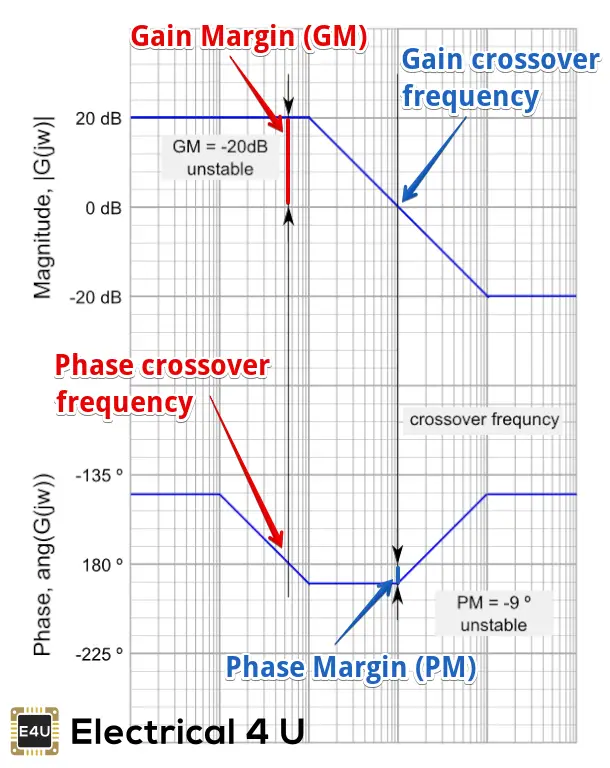
\includegraphics[width=0.68\linewidth]{bode-plot}
	\caption{}
	\label{fig:bode-plot}
\end{figure}


\end{frame}





\begin{frame}{Bode plot with resonance, 1}
	\begin{flushleft}
	
Consider a system with resonance:
%
\begin{equation}
	\begin{cases}
		\dot{\bo{x}} = 
		\begin{bmatrix}
			0 & 1 \\
			-1 & 0
		\end{bmatrix}
		\bo{x}
		+ 
		\begin{bmatrix}
			0\\
			1
		\end{bmatrix}
		\bo{u} 
		\\
		\bo{y} = 
		\begin{bmatrix}
			1 & 0
		\end{bmatrix}
		\bo{x}
	\end{cases}
\end{equation}

The state matrix of this system has eigenvalues $\lambda_i = \pm j$ with resonance frequency $\omega = 1$.

\bigskip

The eigenvalues of the closed-loop system $\bo{A} - \bo{B} \bo{C}$ are $\lambda_i = \pm \sqrt{2} j$ with resonance frequency $\omega = \sqrt{2}$.

\end{flushleft}
\end{frame}



\begin{frame}{Bode plot with resonance, 2}
	% \framesubtitle{O}
	
	% credit: https://www.electrical4u.com/bode-plot-gain-margin-phase-margin/
	\begin{figure}
		\centering
		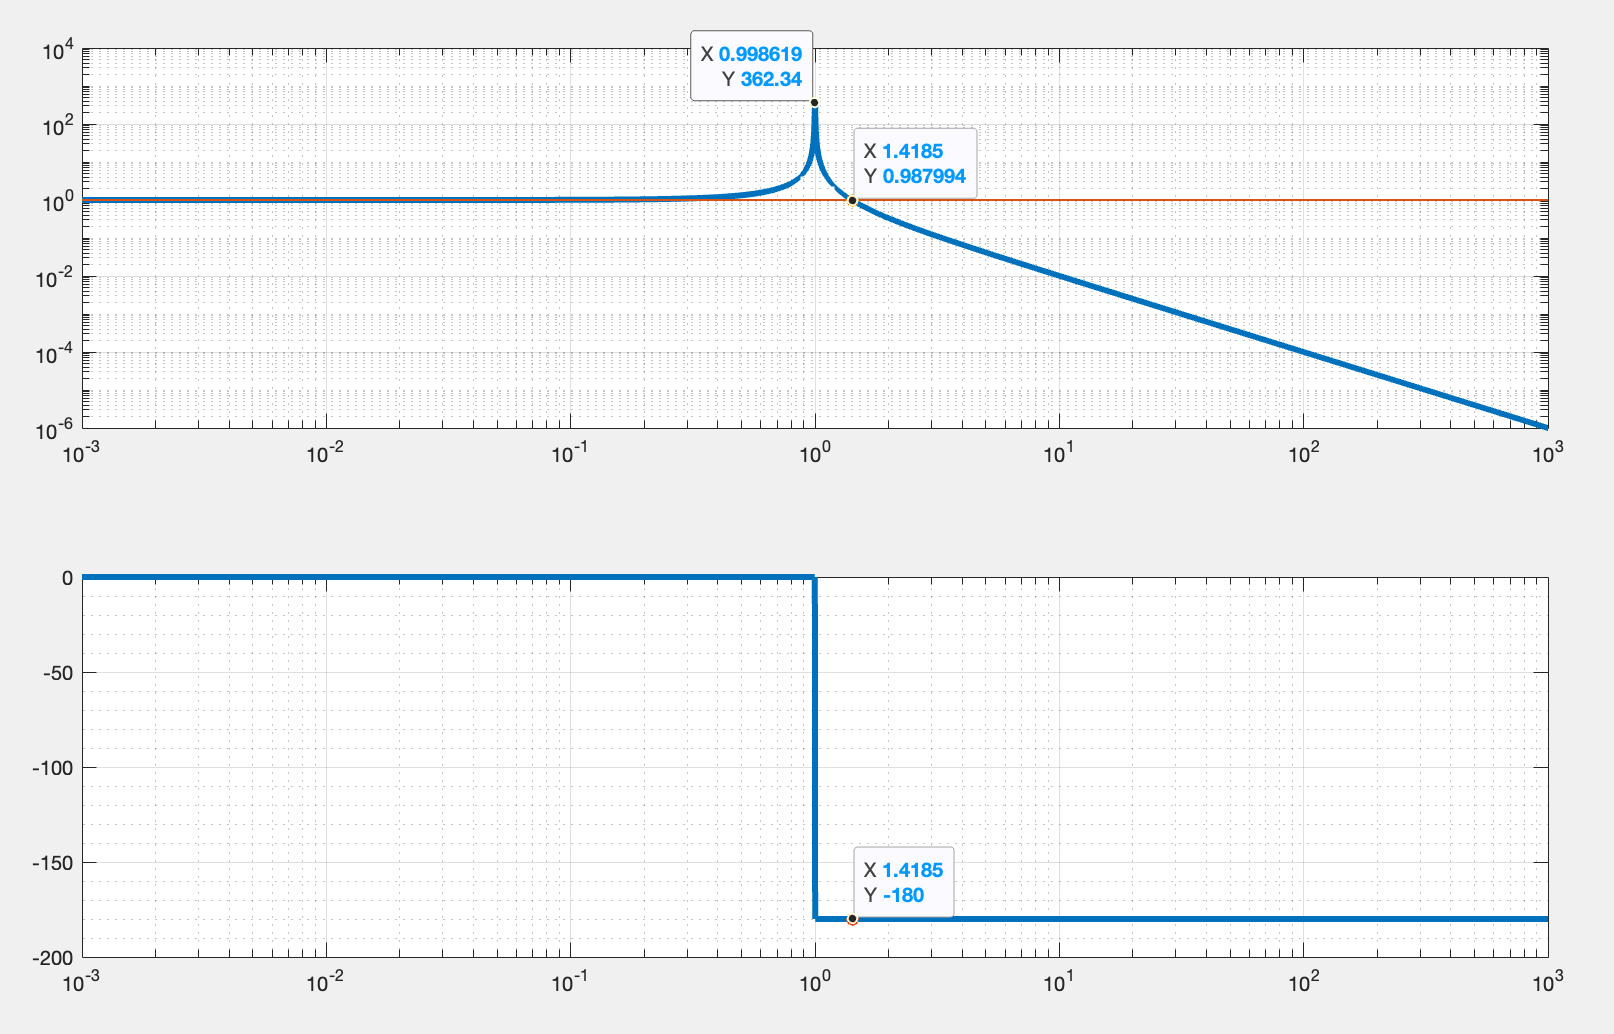
\includegraphics[width=0.95\linewidth]{Resonance}
		\caption{Bode plot of a system with resonance}
		\label{fig:Resonance}
	\end{figure}
	
	
\end{frame}



\begin{frame}{Literature}

\begin{itemize}
	
	
\item Nise, N.S. Control systems engineering. John Wiley \& Sons. (Chapter 10 Frequency Response Techniques)	
	

\item \bref{https://control.asu.edu/Classes/MAE318/318Lecture18.pdf}{Matthew M. Peet; Systems Analysis and Control - Lecture 18: The Frequency Response}	
	
	
\item \bref{https://youtu.be/_eh1conN6YM}{Control System Lectures - Bode Plots, Introduction}

\item \bref{https://global.oup.com/us/companion.websites/fdscontent/uscompanion/us/static/companion.websites/9780199339136/Appendices/Appendix_F.pdf}{Oxford University Press. s-Domain analysis: poles, zeros, and Bode plots}


\end{itemize}

\end{frame}




\myqrframe




\begin{frame}{Laplace and Fourier transforms}
	% \framesubtitle{O}
	\begin{flushleft}
		
		\begin{itemize}
			\item \emph{Fourier series} can be seen as representing a periodic function as a sum of harmonics (sines and cosines). These sines and cosines can be thought of as forming a basis in a linear space. The coefficients of the series can be thought of as a discrete spectrum of the function.
			
			\item \emph{Fourier transform} gives a continuous spectrum of the function. The "basis" is still made of harmonic functions.
			
			\item \emph{Laplace transform} also gives a continuous spectrum of the function, but in a different basis: the basis is given by complex exponentials. I like to think of this basis as solutions of second order ODEs.
		\end{itemize}
		
	\end{flushleft}
\end{frame}



\begin{frame}{Laplace and Fourier transforms}
	% \framesubtitle{O}
	\begin{flushleft}
		
		Let's compare. Fourier transform:
		
		\begin{equation}
			F(\omega) = \int_{-\infty}^\infty f(t) e^{-2\pi j t \omega} dt, \ \ \omega \in \mathbb{R}
		\end{equation}
		
		Laplace transform:
		
		\begin{equation}
			F(s) = \int_0^\infty f(t) e^{-st}dt, \ \ s \in \mathbb{C}
		\end{equation}
		
		We can see that Fourier looks like Laplace with purely imaginary number in the exponent.
		
	\end{flushleft}
\end{frame}



\begin{frame}{Laplace and steady state solution}
	% \framesubtitle{O}
	\begin{flushleft}
		
		From analysing solutions of linear ODEs we know that, given harmonic input (sine, cosine, their combination) "after the transient process is over, the solution approaches a harmonic with the same frequency", but possibly different amplitude and phase.
		
		\bigskip
		
		Intuitively we can think of the imaginary part of $s$ as having to do with this frequency response. 
		
		\bigskip
		The kernel function of the Laplace transform is $e^{-st}$ with $s = \sigma + j \omega$ being a complex variable. If $\sigma = 0$, the kernel becomes $e^{-j \omega t} = \text{cos}(\omega t) - j \text{sin}(\omega t)$. You can see the similarity with Fourier transform kernel.
		
		
	\end{flushleft}
\end{frame}




\end{document}
